\begin{figure}[bt!]
\centering
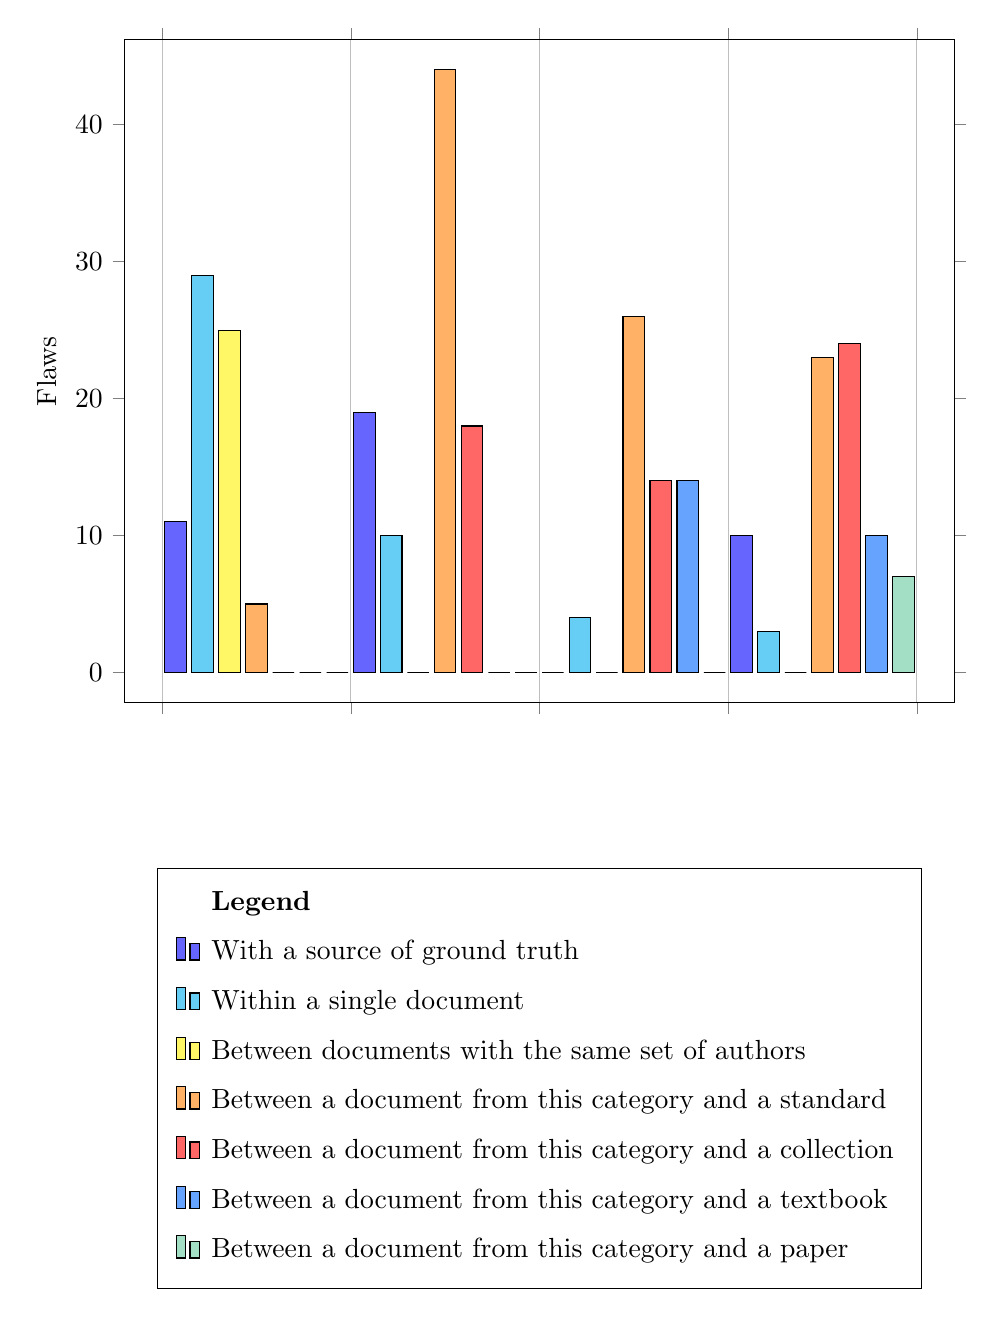
\begin{tikzpicture}
\begin{axis}[
width=\textwidth, height=10cm,
symbolic x coords={std,meta,text,paper,infer},
x tick label as interval,
xticklabels={{\parbox{0.16\textwidth}{\centering \stds{}}},{\parbox{0.16\textwidth}{\centering \metas{}}},{\parbox{0.16\textwidth}{\centering \texts{}}},{\parbox{0.16\textwidth}{\centering \papers{}}},{\parbox{0.16\textwidth}{\centering \infers{}}}},
ylabel=Flaws,
enlargelimits=0.05, xbar=0pt, ybar interval=0.8,
legend style={at={(0.5,-0.25)}, anchor=north, legend columns=1,
inner xsep=6pt,inner ysep=4pt,
nodes={inner sep=4pt,text depth=0.3em},},
legend cell align=left,
]
\addlegendimage{empty legend}
\addplot[fill=blue!60] coordinates {(std, 11) (meta, 19) (text, 0) (paper, 10) (infer, 0)};
\addplot[fill=cyan!60] coordinates {(std, 29) (meta, 10) (text, 4) (paper, 3) (infer, 0)};
\addplot[fill=yellow!60] coordinates {(std, 25) (meta, 0) (text, 0) (paper, 0) (infer, 0)};
\addplot[fill=orange!60] coordinates {(std, 5) (meta, 44) (text, 26) (paper, 23) (infer, 0)};
\addplot[fill=red!60] coordinates {(std, 0) (meta, 18) (text, 14) (paper, 24) (infer, 0)};
\addplot[fill=blue!60!cyan!60] coordinates {(std, 0) (meta, 0) (text, 14) (paper, 10) (infer, 0)};
\addplot[fill=cyan!60!yellow!60] coordinates {(std, 0) (meta, 0) (text, 0) (paper, 7) (infer, 0)};
\addlegendentry{{\centering \textbf{Legend}}}
\addlegendentry{With a source of ground truth}
\addlegendentry{Within a single document}
\addlegendentry{Between documents with the same set of authors}
\addlegendentry{Between a document from this category and a standard}
\addlegendentry{Between a document from this category and a collection}
\addlegendentry{Between a document from this category and a textbook}
\addlegendentry{Between a document from this category and a paper}
\end{axis}
\end{tikzpicture}
\caption{Identified flaws by the \hyperref[sources]{source tier} responsible.}
\label{fig:flawBars}
\end{figure}
